\documentclass[12pt, a4]{article}
\usepackage[margin=2cm]{geometry}
\usepackage{parskip}
\usepackage{nameref}
\usepackage{enumitem}
\usepackage{tabularx}
\usepackage{hyperref}
\usepackage[tiny]{titlesec}

\usepackage{amsmath}
\usepackage{amssymb}

\usepackage{fancyhdr}
\usepackage{titling}

\usepackage{pgfplots}
\pgfplotsset{compat=1.16}
\usetikzlibrary{decorations.pathreplacing,positioning, shapes,arrows,chains}


\usepackage{xcolor}
\usepackage{graphicx}
\usepackage{fancyvrb}
\usepackage{listings}
\usepackage{bm}
\usepackage{xcolor}
\usepackage{optidef}

\usepackage{pifont} % for cmark and xmark
\newcommand{\cmark}{\ding{51}}%
\newcommand{\xmark}{\ding{55}}%
\newcommand{\checkedbox}{\rlap{$\square$}{\raisebox{2pt}{\hspace{1pt}\cmark}}}
%\newcommand{\crossedBox}{\rlap{$\square$}{\large\hspace{1pt}\xmark}}


\xdefinecolor{gray}{rgb}{0.4,0.4,0.4}
\xdefinecolor{blue}{RGB}{58,95,205}
\xdefinecolor{darkgreen}{RGB}{0,100,0}

\newcommand{\lightgray}{black!30}

\newcommand{\plotDomain}{-1:8}

\newcommand{\addPlotLDownCoords}[1]{
	\addplot[mark=none, domain=\plotDomain, color=\lightgray,
	decoration={border,segment length=1mm,amplitude=1.5mm,angle=-135},
	postaction={decorate}
	] coordinates {#1};
	\addplot[mark=none, domain=\plotDomain] coordinates {#1};
}

\newcommand{\addPlotLDown}[1]{
	\addplot[mark=none, domain=\plotDomain, color=\lightgray,
	decoration={border,segment length=1mm,amplitude=1.5mm,angle=-135},
	postaction={decorate}
	] {#1};
	\addplot[mark=none, domain=\plotDomain] {#1};
}

\newcommand{\addPlotRUpCoords}[1]{
	\addplot[mark=none, domain=\plotDomain, color=\lightgray,
	decoration={border,segment length=1mm,amplitude=1.5mm,angle=135},
	postaction={decorate}
	] coordinates {#1};
	\addplot[mark=none, domain=\plotDomain] coordinates {#1};
}

\newcommand{\addPlotRUp}[1]{
	\addplot[mark=none, domain=\plotDomain, color=\lightgray,
	decoration={border,segment length=1mm,amplitude=1.5mm,angle=135},
	postaction={decorate}
	] {#1};
	\addplot[mark=none, domain=\plotDomain] {#1};
}

\lstset{% setup listings
	language=R,% set programming language
	basicstyle=\ttfamily\small,% basic font style
	keywordstyle=\color{blue},% keyword style
	commentstyle=\color{gray},% comment style
	numbers=left,% display line numbers on the left side
	numberstyle=\scriptsize,% use small line numbers
	numbersep=10pt,% space between line numbers and code
	tabsize=3,% sizes of tabs
	showstringspaces=false,% do not replace spaces in strings by a certain character
	captionpos=b,% positioning of the caption below
	breaklines=true,% automatic line breaking
	escapeinside={(*}{*)},% escaping to LaTeX
	fancyvrb=true,% verbatim code is typset by listings
	extendedchars=false,% prohibit extended chars (chars of codes 128--255)
	literate={"}{{\texttt{"}}}1{<-}{{$\bm\leftarrow$}}1{<<-}{{$\bm\twoheadleftarrow$}}1
	{~}{{$\bm\sim$}}1{<=}{{$\bm\le$}}1{>=}{{$\bm\ge$}}1{!=}{{$\bm\neq$}}1{^}{{$^{\bm\wedge}$}}1,% item to replace, text, length of chars
	alsoletter={.<-},% becomes a letter
	alsoother={$},% becomes other
	otherkeywords={!=, ~, $, \&, \%/\%, \%*\%, \%\%, <-, <<-, /},% other keywords
	deletekeywords={c}% remove keywords
}



\author{Pascal Lüscher}
\title{Mathematical Optimization – Problem set 6}

\makeatletter
\let\mytitle\@title
\makeatother

\pagestyle{fancy}
\fancyhf{}
\rhead{
	\mytitle\\
	\theauthor
}

\rfoot{
	Page: \thepage
}

\renewcommand{\arraystretch}{1.2} % more space in tables
\renewcommand\thesubsection{\thesection.\alph{subsection}}
\titleformat{\section}[hang]{\normalfont\bfseries\itshape}{\textup{\thesubsection}}{1em}{}

\titleformat{\subsection}[hang]{\normalsize\itshape}{\textup{\thesubsection}}{1em}{}[]

\newcommand{\norm}[1]{\lvert #1 \rvert}

\newcolumntype{L}{>{$}l<{$}} % math-mode version of "l" column type
\newcolumntype{R}{>{$}r<{$}} % math-mode version of "l" column type
\newcolumntype{C}{>{$}c<{$}} % math-mode version of "l" column type


\begin{document}
	\section{Problem 1: Complementary slackness}
	Consider the following linear program in canonical form
	\begin{equation}\label{eq:prob1_canonical}
		\begin{array}{lrcrcrcrcrcrcrr}
			\text{max}  &      &   & 4x_2 & + & 2x_3 & - &  x_4 & + & 3x_5 & - & 7x_6 \\
			\text{s.t.} &  x_1 &   &      &   &      & - &  x_4 &   &      & + & 3x_6 & \leq & -1 \\
						& 7x_1 & + &  x_2 & + &  x_3 &   &      & + &  x_5 & + &  x_6 & \leq &  5 \\
			  			&      &   &  x_2 & - &  x_3 &   &      &   &      & - &  x_6 & \leq &  1 \\
						&      &   &  x_2 & - &  x_3 & + &  x_4 & + &  x_5 & + &  x_6 & \leq &  5 \\
			 			&  x_1 &   &      & + &  x_3 & - & 4x_4 & + & 5x_5 &   &      & \leq &  0 \\
			            &      &   &      &   &      &   &      &   &      &   &  x_i & \geq & 0 & \forall i \in \{1,\ldots,6\}
		\end{array}
	\end{equation}
\subsection{Write the dual of the above linear program.}
	 \begin{equation}\label{eq:prob1_dual}
 		\begin{array}{lcrcrcrcrcrcrr}
 			\text{min}  & - &  y_1 & + & 5y_2 & + &  y_3 & + & 5y_4 &  &  \\
 			\text{s.t.} &   &  y_1 & + & 7y_2 &   &      &   &      & + &  y_5 & \geq &  0\\
 					 	&   &      &   &  y_2 & + &  y_3 & + &  y_4 &   &      & \geq &  4\\
 					 	&   &      &   &  y_2 & - &  y_3 & - &  y_4 & + &  y_5 & \geq &  2\\
 					 	& - &  y_1 &   &      &   &      & + &  y_4 & - & 4y_5 & \geq & -1\\
 					 	&   &      &   &  y_2 &   &      & + &  y_4 & + & 5y_5 & \geq &  3\\
 					 	&   & 3y_1 & + &  y_2 & - &  y_3 & + &  y_4 &   &      & \geq & -7\\
 					 	&   &      &   &      &   &      &   &      &   &  y_i & \geq & 0 & \forall i \in \{1,\ldots,5\}\\
 		\end{array}
 	\end{equation}
 
\subsection{Consider the primal feasible solutions}
\begin{equation*}
	x^*=\begin{pmatrix}
		0 \\ 2 \\ 2 \\ 4 \\ 0 \\ 1
		\end{pmatrix}
	\quad\quad\text{and}\quad\quad
	x^*=\begin{pmatrix}
		0 \\ 3 \\ 2 \\ 1 \\ 0 \\ 0
	\end{pmatrix}
\end{equation*}
Use the complementary slackness theorem (Theorem 1.90 in the script) to decide whether these two candidates are optimal solutions of the given linear program.

\subsubsection{First $x^*$}
The objective value for the primal solution $x^*$ is $4\cdot2 + 2\cdot2 -4 - 7 = 1$.
We first need to derive the dual solution.
$y^* = \begin{pmatrix} 0 \\ 0 \\ 2 \\ 0 \\ 14 \end{pmatrix}$ which yields the objective value $2$. $2 \neq 1$ and therefore is $x^*$ not optimal.
\subsubsection{Second $x^*$}
The objective value for the primal solution $x^*$ is $3\cdot4 + 2\cdot2 - 1 = 15$
We first need to derive the dual solution
$y^* = \begin{pmatrix} 0 \\ 0 \\ 0 \\ 3 \\ 2 \end{pmatrix}$ yields the objective value $15$. $15 = 15$ and therefore is $x^*$ is optimal.

\section{Problem 2: Asymptotic growth and Landau notation}
Indicate whether the following statements are true or false by ticking the right box. Additionally, provide a short justification of your answer (the given space should be enough).
\subsection{Let $f(n) = \log(n^2)$ and $g(n) = \log(n)$. Then $f= \Theta(g)$}

True \checkedbox\quad False $\square$

Short justification: Since $\log(n^2) = 2 \log(n)$, $f(n)$ grows faster by a constant factor of $2$.

\subsection{Let $f(n) = n+\sqrt{n}$ and $g(n) = n\log(n)$. Then $f=O(g)$.}
True \checkedbox\quad False $\square$

Short justification: $n + \sqrt{n} < n\log(n)$ and therefore $f(n) < g(n)$.

\subsection{Let $f(n) = 2^n$ and $g(n) =n!$. Then $f= \Theta(g)$.}
True $\square$\quad False \checkedbox

Short justification: $n!$ grows faster than $2^n$

\subsection{Let $f(n) =\sqrt{n}^n$ and $g(n) =n^{\sqrt{n}}$. Then $f= \Theta(g)$.}
True $\square$\quad False \checkedbox

Short justification: $\sqrt{n}^n = n^{\frac{n}{2}}$ and $n^{\sqrt{n}} = n^{n^\frac{1}{2}}$. Clearly $\frac{n}{2}$ does not grow the same as $n^\frac{1}{2}$.

\subsection{Let $f(n) = 3^n$ and $g(n) = 2^{n+\log n}$. Then $f= \Omega(g)$}.
True \checkedbox\quad False $\square$

Short justification: $3^n$ grows faster than $2^{n+\log n}$

\subsection{Let $f, g:\mathbb{Z}_{\geq1} \rightarrow \mathbb{Z}_{\geq1}$. Then, at least one of the relations $f=O(g),g=O(f)$, or $f= \Theta(g)$ holds.}
True \checkedbox\quad False $\square$

Short justification: If $f$ grows faster than $g$, $f=O(g)$ holds. If $g$ grows faster than $f$, $g=O(f)$ holds. If both grow equally fast $f=\Theta(g)$ holds.

\section{Problem 3: Running time of a sorting algorithm}
$\ldots$ insertion sort $\ldots$

Implementation (simplified for myself)
\begin{lstlisting}[language={[Sharp]c}]
InsertionSort(int[] A) {
	for (int i = 1; i < A.length; ++i) {
		int j = i;
		while (j >= 1 && A[j-1] > A[j]) {
			int x = A[j];
			A[j] = A[j-1];
			A[j-1] = x;
			j--;
		}
	}
	return A;
}
\end{lstlisting}

\subsection{Track how a call of Algorithm 1 on the array $A= [4,3,1,2]$ changes $A$}
$[4,3,1,2]$\\
$[3,4,1,2]$\\
$[3,1,4,2]\quad[1,3,4,2]$\\
$[1,3,2,4]\quad[1,2,3,4]$

\subsection{Prove that Algorithm 1 has a worst-case running time of $O(n^2)$.}
Worst case scenario is with a reverse-sorted array. In this case it performs $i$ steps $i$ times. Therefore the running time is $i\cdot i = i^2 = O(n^2)$

\subsection{Show that Algorithm 1 has a running time of $\Omega(n^2)$ on some inputs}
$A = [4,3,2,1]$

\subsection{Show that there exist inputs on which Algorithm 1 has a running time of only $O(n)$.}
Sorted array $A = [1,2,3,4]$

\section{Problem 4: Quering edge existence in incidence lists}
Let $G= (V, E)$ be a graph given by an incidence list and let $u, v\in V$ two vertices. Show that in time $O(\min\{deg(u),deg(v)\})$, it can be decided whether $G$ contains an edge $\{u, v\}$.

The edge $\{u,v\}$ is contained in the list for $u$ and in the list for $v$. An algorithm with running time of $O(2\cdot\min\{deg(u),deg(v)\})$ woks as the following:
\pagebreak
\begin{lstlisting}
ContainsEdge(u, v) {
	var currentUEdge = u.FirstEdge;
	var currentVEdge = v.FirstEdge;
	while(true) {
		if (currentUEdge.Start == v || currentUEdge.End == v) {
			return true;
			if (!currentUEdge.Next()) {
				return false;
			}
			currentUEdge = currentUEdge.Next();
		}
		if (currentVEdge.Start == u || currentVEdge.End == u) {
			return true;
			if (!currentVEdge.Next()) {
				return false;
			}
			currentVEdge = currentVEdge.Next();
		}
	}
}
	
\end{lstlisting}

\pagebreak
\section{Problem 5: Meeting at a central point}
Imagine three caterpillars sitting on vertices $v1,v2,$ and $v3$ of a connected graph $G= (V, E)$. The three caterpillars would like to meet at one of the vertices of the graph. All they can do is moving from one vertex to another via the edges of the graph, and they can only stop at vertices of the graph,but not on an edge. When traversing an edge, the three caterpillars travel at the same speed of one edge per hour.

 For an example, consider \autoref{fig:graph_caterpillar}. To meet at vertex $v5$, the caterpillar from vertex $v1$ could travel to $v5$ via the vertices $v4$ and $v2$ in three hours (and there is no faster option), and the caterpillars from $v2$ and $v3$ could be there in one and two hours, respectively. Thus, an earliest meeting at $v5$ could take place three hours after the caterpillars start moving.
 
 \begin{figure}[h]
 	\centering
 	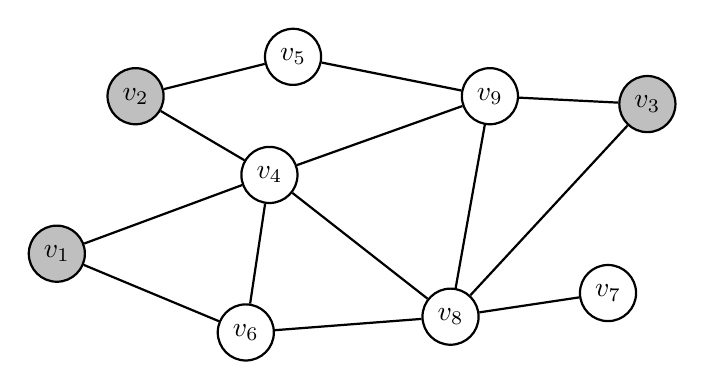
\begin{tikzpicture}
 		\begin{scope}[every node/.style={circle,thick,draw}]
 			\node[fill=lightgray] (v1) at (0,0) {$v_1$};
 			\node[fill=lightgray] (v2) at (1,2) {$v_2$};
			\node (v4) at (2.7,1) {$v_4$};
			\node (v5) at (3,2.5) {$v_5$};
			\node (v6) at (2.4,-1) {$v_6$};
			\node (v8) at (5, -.8) {$v_8$};
			\node (v9) at (5.5, 2) {$v_9$};
			\node[fill=lightgray] (v3) at (7.5, 1.9) {$v_3$};
			\node (v7) at (7, -.5) {$v_7$};
 		\end{scope}
	 	\begin{scope}[every path/.style={thick}]
			\path (v1)  edge (v4) edge (v6);
			\path (v2) edge (v5) edge (v4);
			\path (v4) edge (v6) edge (v8) edge (v9);
			\path (v5) edge (v9);
			\path (v8) edge (v6) edge (v9) edge (v3) edge (v7);
			\path (v3) edge (v9);
	 	\end{scope}
	\end{tikzpicture}
	\caption{A graph $G= (V, E)$ with starting points of the caterpillars marked in gray.}
	\label{fig:graph_caterpillar}
\end{figure}
 
 Of course, the caterpillars want to meet at a vertex where an earliest possible meeting can be achieved. Can you provide an algorithm that determines such a vertex?  Analyze the running time of your algorithm. Is it possible to construct an algorithm that solves the given problem and has running time $O(|V|+|E|)$?
 

 Algorithm idea in words:
 It's a BFS algorithm, we cycle through the caterpillars last visited Verteces and move 1 further. If we get to an edge where all 3 caterpillars join, we have found the minimum point. To simplify the technical details, the class \emph{Vertex} is given as the following:
 \begin{lstlisting}[language={[Sharp]c}] 		
 	class Vertex {
 		public int?[] Distance = new int?[caterpillars.Count];
 		public Vertex[] adjacentVerteces();
 	}
 \end{lstlisting}
and \emph{caterpillars} is an array of the class \emph{Caterpillar} given as the following:
 \begin{lstlisting}[language={[Sharp]c}] 		
	class Caterpillar {
		public Vertex StartingVertex;
	}
\end{lstlisting}

\pagebreak
 Algorithm:
 \begin{lstlisting}[language={[Sharp]c}] 
	var latestCaterpillarVertices = new Vertex[caterpillars.Count][]
 	for (var i = 0; i < caterpillars.Count; ++i) {
 		latestCaterpillarVertices[i] = new [] {caterpillars[i].StartingVertex};
 	}
 	
 	currDistance = 0;
	while (true) {
 		currDistance++;
	 	for (var i = 0; i < caterpillars.Count; ++i) {
	 		var newLatestCaterpillarVertices = [];
	 		
			foreach (var vertex in latestCaterpillarVertices[i]) {
				foreach (var adjacentVertex in vertex.adjacentVerteces()) {
					if (null == adjacentVertex.Distances[i]) {
						// vertex not yet visited
						adjacentVertex.Distances[i] = currDistance;
						newLatestCaterpillarVertices.Add(adjacentVertex);
						
						// check break condition
						meetingPointFound = true;
						for (var j = 0; j < caterpillars.Count; ++j) {
							meetingPointFound &= null != adjacentVertex.Distances[i];						
						}
						if (meetingPointFound) {
							return adjacentVertex;
						}
					}
				}
			}
			latestCaterpillarVertices[i] = newLatestCaterpillarVertices;
		}
	}
 \end{lstlisting}

The running time is $O(\#caterpillars \cdot (|V| + |E|))$


\end{document}